\documentclass[../slides.tex]{subfiles}
\begin{document}

\begin{frame}{Digitalisierung: Bauteil}
    \begin{minipage}[t]{.39\textwidth}
      \begin{itemize}
        \item Scanner: Micro-Epsilon, LLT3000-25
        \item Limitierter Messbereich
        \item Limiterte Auflösung und Genauigkeit
        \item Scanergebnis mit 13205223 Polygonen
        \item Pre-Processing
        \item Top-Down Ansicht erstellen
      \end{itemize}
    \end{minipage}
    \hfill
    \begin{minipage}[t]{.6\textwidth}
      \begin{figure}[]
        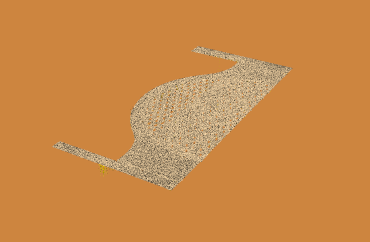
\includegraphics[height=140pt]{img_niklas/base_scan.png}
        \caption{Scanergebnis}
        \label{fig:base_scan}
        %
      \end{figure}
    \end{minipage}
  \end{frame}

  \begin{frame}{Digitalisierung: Stitching}
    \begin{minipage}[]{.49\textwidth}
        \begin{figure}[]
            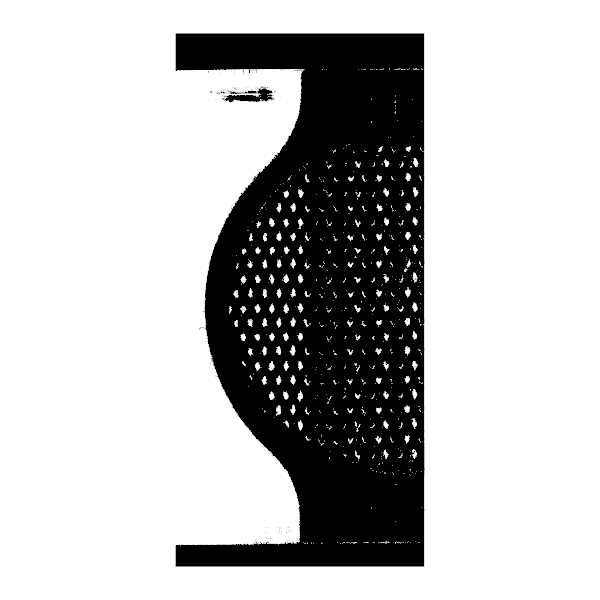
\includegraphics[width=150pt]{img_niklas/scanner_2.png}
            \caption{Scanner TOP-DOWN Ansicht links (generiert)}
            \label{fig:scanner_left}
          \end{figure}
    \end{minipage}
    \hfill
    \begin{minipage}[]{.49\textwidth}
      \begin{figure}[]
        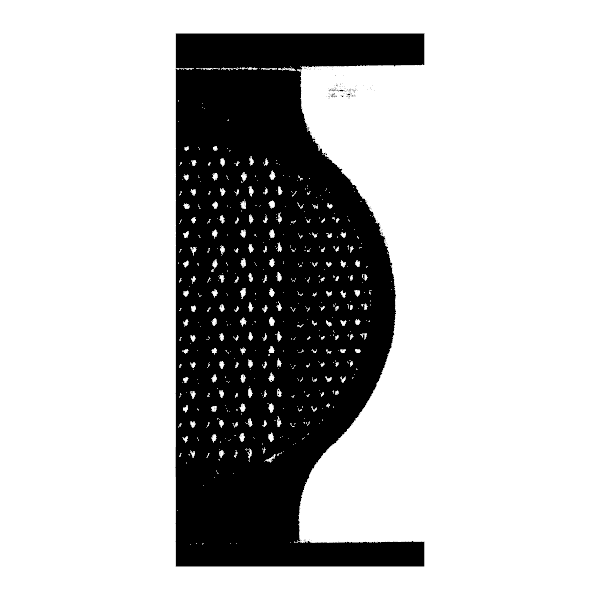
\includegraphics[width=150pt]{img_niklas/scanner_1.png}
        \caption{Scanner TOP-DOWN Ansicht rechts (generiert)}
        \label{fig:scanner_right}
      \end{figure}
    \end{minipage}
  \end{frame}


\end{document}